
\includegraphics[height=1.25cm]{images/pictograms/replication}
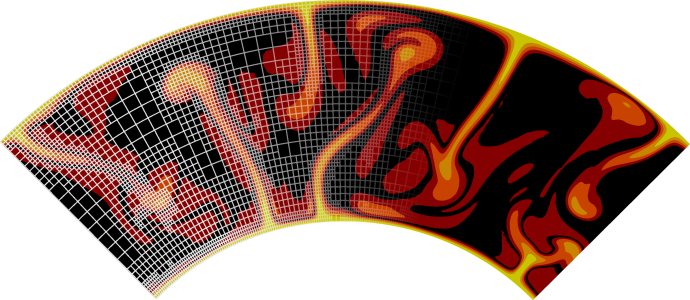
\includegraphics[height=1.25cm]{images/pictograms/aspect_logo}

\includegraphics[height=1.25cm]{images/pictograms/benchmark}

\includegraphics[height=1.25cm]{images/pictograms/under_construction}

\includegraphics[height=1.25cm]{images/pictograms/FEM}
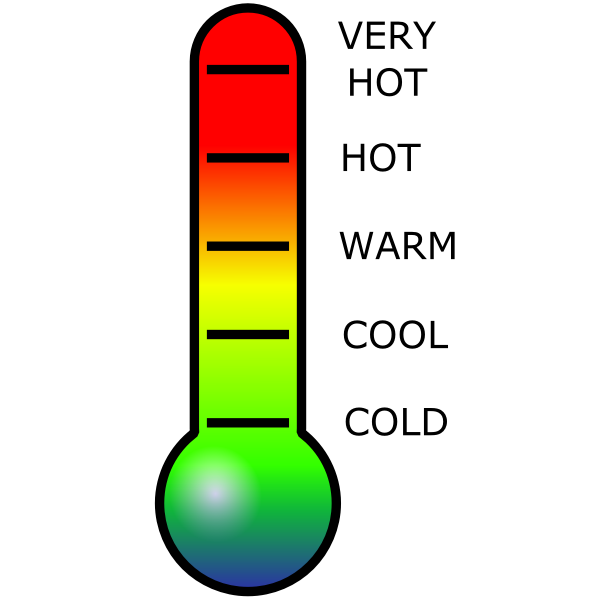
\includegraphics[height=1.25cm]{images/pictograms/temperature}

%%%%%%%%%%%%%%%%%%%%%%%%%%%%%%%%%%%%%%%%%%%%%%%%%%%%%%%%%%%%%%%%%%%%%%%%%%%%%%%%%%%%%%%%%%%%%%%%%%%

\begin{flushright} {\tiny {\color{gray} python\_codes/fieldstone\_149/text.tex}} \end{flushright}

\lstinputlisting[language=bash,basicstyle=\small]{python_codes/fieldstone_149/keywords.key}

\par\noindent\rule{\textwidth}{0.4pt}

\begin{center}
\inpython
{\small Code: \url{https://github.com/cedrict/fieldstone/tree/master/python_codes/fieldstone_149}}
\end{center}

\par\noindent\rule{\textwidth}{0.4pt}

{\sl This stone was developed in with input from Daniel Douglas}. 

\par\noindent\rule{\textwidth}{0.4pt}

%%%%%%%%%%%%%%%%%%%%%%%%%%%%%%%%%%%%%%%%%%%%%%%%%%%%%%%%%%%%%%%%%%%%%%%%%%%%%%%%%%%%%%%%%%%%%%%%%%%

%-------------------------------------
\section*{Joining two simple and identical meshes}

This is implemented in { stone1.py}

%-------------------------------------
\section*{Joining multiple meshes}

This proto-mesh contains 8 elements and 14 points.

\begin{verbatim}
12---------------13
| \               |
|  10------------11
|   | \           |
|   |  \          |
|   |   \         |
|   |    \        |
5---6     8-------9       
|   | \-  / \     |
|   |   7-   \    |
|   |     \   \   |
0---1-----2----3--4
\end{verbatim}

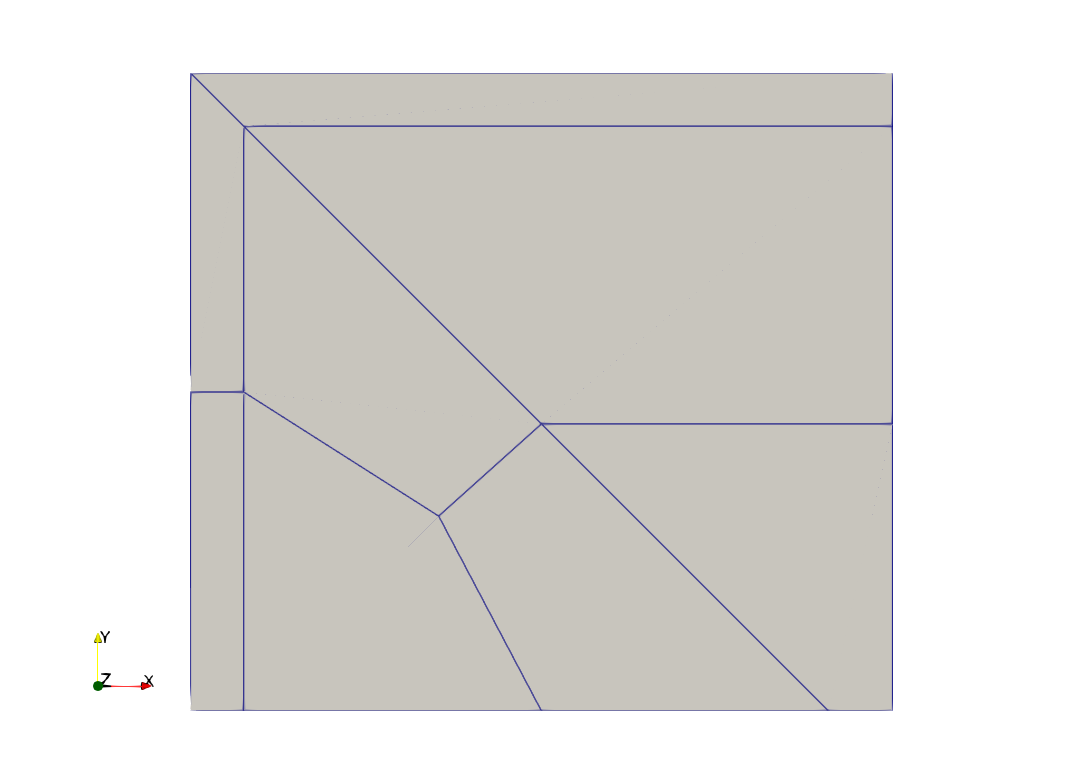
\includegraphics[width=8cm]{python_codes/fieldstone_149/mesh}

We then proceed by creating 8 blocks. We then map them and finally 
assemble them one by one.



%%%%%%%%%%%%%%%%%%%%%%%%%%%%%%%%%%%%%%%%%%%%%%%%%%%%%%%%%%%%%%%%%%%%%%%%%%%%%%%%%%%%%%%%%%%%%%%%%%%
\par\noindent\rule{\textwidth}{0.4pt}

\vspace{.5cm}

\begin{center}
\fbox{\begin{minipage}{0.9\textwidth}
{\color{teal}To Do, open questions, future work?}
\begin{itemize}
\item 
what i want to do is implement an algo which adds nodes 
to the original patch of cells.

\item use f131 P1 to P2 tool to make Q1 to Q2 
\end{itemize}
\end{minipage}}
\end{center}

%%%%%%%%%%%%%%%%%%%%%%%%%%%%%%%%%%%%%%%%%%%%%%%%%%%%%%%%%%%%%%%%%%%%%%%%%%%%%%%%%%%%%%%%%%%%%%%%%%%
\vspace{.5cm}

\Literature:\\
\fullcite{vack08}\\
\fullcite{vatc23}

